\chapter{Описание и реализация нового алгоритма недоминирующей сортировки ENS-NDT-ONE}
\label{chapter3}

В данной главе описан новый алгоритм ENS-NDT-ONE, который лучше подходит на роль одного из алгоритмов, на основе которых был разработан гибридный алгоритм. Также в данной главе представлена и доказана асимптотическая оценка времени работы алгоритма ENS-NDT-ONE.

\section{Описание алгоритма}

Причины, по которым алгоритм Роя и алгоритм Густавссона не подходили для создания эффективного гибридного алгоритма (см Главу~\ref{chapter2}), породили необходимость в создании нового алгоритма недоминирующей сортировки. В результате нами был разработан алгоритм ENS-NDT-ONE. Разработанный алгоритм по большей части основан на идеях алгоритма Густавсона, но при этом структура данных, используемая в нем значительно модифицирована. Это позволило избежать необходимости перебора всех $k$-$d$ деревьев.

Алгоритм ENS-NDT был изменен следующим образом: вместо множества деревьев теперь хранится одно дерево для всех точек. Именно по этой причине алгоритм назван ENS-NDT-ONE. Параметрами дерева, как и в оригинальной версии алгоритма, будет размер корзины, ограничивающий максимальное число точек, которое может содержаться в одной вершине, и глубина, начиная с которой размер корзины игнорируется, и точки перестают делиться на две при превышении первого порога. Так же, как в оригинальном алгоритме, дерево будет сбалансированным. Это обеспечивается предварительно подсчитанной структурой $split$. На Рисунке~\ref{ndtree_new} представлена схема структуры данных, поддерживаемой в алгоритме ENS-NDT-ONE.

\begin{figure}[!h]
\begin{center}
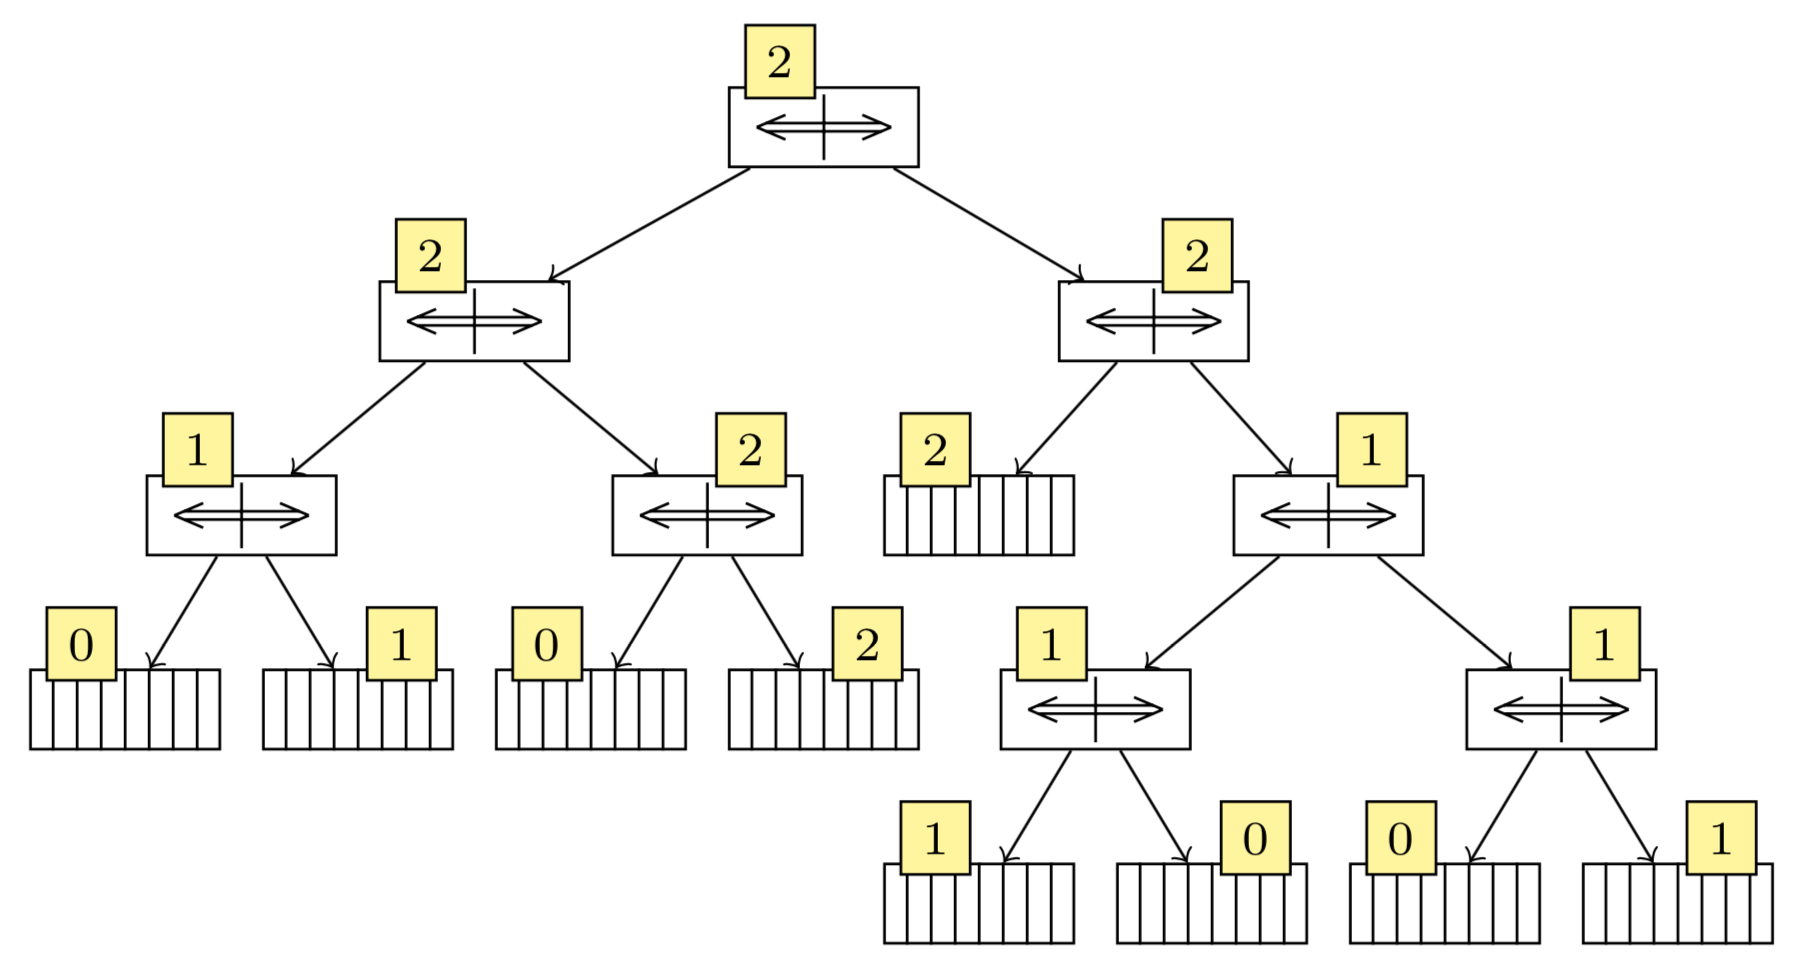
\includegraphics[width=15cm]{pic/ndtree_new.png}
\caption{Пример $k$-$d$ дерева с максимальными рангами на поддеревьях, которое поддерживается алгоритм ENS-NDT-ONE}.
\label{ndtree_new}
\end{center}
\end{figure}

Одной из причин высокой производительности алгоритма ENS-NDT является то, что, при определении ранга для точки $p$ в некотором дереве, как только найдена точка, доминирующая точку $p$, можно сразу же убрать из рассмотрения это дерево, так как остальные точки из этого дерева не могут влиять на ранг $p$. Такой особенности нет у алгоритма ENS-NDT-ONE, так как в дереве могут встретиться точки с большим или равным рангом, чем ранг рассматриваемой точки $p$.

Чтобы предотвратить потери производительности, мы предлагаем хранить максимальный ранг всех точек на поддереве. Это позволит при определении ранга точки с предпоставленным рангом $k$, не спускаться в поддерево с рангом $\leq k$. На фазе добавления точки в дерево необходимо не забыть обновить значения максимального ранга по пути добавления.

Адаптация алгоритма ENS-NDT-ONE для переключения на него при вызове процедуры $HeplerA$ не требуется, так как при вызове процедуры $HeplerA$ происходит обычная недоминирующая сортировка с небольшим уточнением: при обновлении ранга надо только учитывать предварительный ранг точки и обновлять ранг только в том случае, если он меньше, чем новый ранг. 

Напомним, что процедура $HeplerB$ принимает в качестве аргументов два множества, одно с окончательными рангами $L$, другое предварительными рангами $R$. В процедуре $HeplerB$ происходит обновление рангов множества $R$, по рангам множества $L$. Опишем работу алгоритма ENS-NDT-ONE с двумя множествами $L$ и $R$: 
\begin{enumerate}
  \item Обходим точки в лексикографическом порядке, как в оригинальном алгоритме.
  \begin{enumerate}
      \item Если точка принадлежит множеству с окончательными рангами $L$, добавляем точку в дерево с текущим рангом.
      \item Если точка принадлежит множеству с предварительными рангами $R$, то мы обновляем ранг рассматриваемой точки по дереву и не добавляем ее в структуру, так как ранжирование происходит только на основе точек из множества $L$.
  \end{enumerate}
\end{enumerate}

\section{Асимптотическая оценка времени работы}

Вероятность пропуска поддеревьев сильно влияет на производительность алгоритма ENS-NDT-ONE. В частности, для многих видов входных данных можно показать постоянную верхнюю границу $\alpha$ на вероятность входа в дочерний узел, который соответствует более высокому значению по критерию, рассматриваемому на данном слое. Из этого по Мастер-теореме получаем верхнюю границу $O(MN^{\log_2(1+\alpha)})$ на один запрос к дереву и $O(MN^{1+\log_2(1+\alpha)})$ для времени выполнения всей сортировки, что асимптотически меньше, чем $\Theta(N^2M)$, когда $\alpha<1$. В худшем случае алгоритм ENS-NDT-ONE работает за $O(MN^2)$, однако зачастую время работы алгоритма сильно лучше. Например, когда входные данные состоят из случайно сгенерированных точек в гиперкубе $[0; 1]^M$, существует $O(N)$ точек, при добавлении в k-d дерево которых, вероятность зайти в обоих детей в каждой не листовой вершине дерева не более $1/2$. Таким образом получаем, что верхняя граница асимптотики времени работы равна $O(MN^{1+\log_2(1+1/2)}) \approx O(MN^{1.585})$.

\section{Реализация алгоритма ENS-NDT-ONE}

В данном разделе будет описана реализация алгоритма ENS-NDT-ONE. 

На Листинге~\ref{procedure_end_ndt_one} приведен псевдокод основного метода алгоритма ENS-NDT-ONE, который принимает в качестве аргументов множество точек $P$, $M$ {---} размерность и $B$ {---} порог, максимальное количество точек в вершине. Для получения $split$ структуры используется функция $CreateSplits$, которая описана в Главе~\ref{chapter2} данной работы.

Помимо этого, для ускорения процесса определения ранга, будем хранить максимальный ранг на поддереве, что позволит добавить следующую эвристику: если у поддерева максимальный ранг меньше ранга рассматриваемой точки, то это поддерево никак не может повлиять на ранг данной точки. 

\begin{algorithm}
\begin{algorithmic}[1]
\Procedure{ENS-NDT-ONE}{P, M, B}
    \State{$P \gets Sort(P, a^M \prec b^M, ..., a^1 \prec b^1)$}
    \State{$S \gets CreateSplits(P, M-1,B)$}
    \State{$\mathcal{F} \gets \{\{P_1\}\}$}
    \State{$\mathcal{T} \gets new NDTreeOne(S, B)$}
    \State{$InsertIntoNDTreeOne(\mathcal{T}, P_1)$}
    \State{$j \gets 1$}
    \For{$i = 2, ..., |P|$}
        \If{$P_{i-1} \neq P_{i}$}
            \State {$j \gets FindRankInNDTreeOne(\mathcal{T}, P_i)$}
            \State{$InsertIntoNDTreeOne(\mathcal{T}, \mathcal{P}_i)$}
        \EndIf
        \State{$\mathcal{F}_j \gets \mathcal{F}_j \cup {P_i}$}
    \EndFor
    \State{\Return {$\mathcal{F}$}}
\EndProcedure
\end{algorithmic}
\caption{Главная процедура алгоритма ENS-NDT-ONE.}
\label{procedure_end_ndt_one}
\end{algorithm}

В функцию $FindRankInNDTreeOne$ будет добавлен дополнительный аргумент, ранг точки $P_i$, тогда функция $FindRankInNDTreeOne$ в листовой вершине будет иметь реализацию представленную на Листинге~\ref{procedure_find_rank_term}. А в узловой вершине реализация представляет из себя два рекурсивных вызова на вершинах-потомках с одним только отсечением, если координата рассматриваемой вершины больше либо равна медианному значению, то в левого ребенка можно не заходить, потому что в поддерево, где по текущей координате все точки больше рассматриваемой, не найдется ни одной точки, которая бы доминировала нашу. На Листинге~\ref{procedure_find_rank_n_term} представлен псевдокод определения ранга в узловой вершине.

\begin{algorithm}
\begin{algorithmic}[1]
\Procedure{FindRankInNDTreeOne}{$\mathcal{T}, p, r$}
    \If {$ maxRank < r$}
        \State {\Return {r}}
    \EndIf

    \If{$p[\mathcal{T}.splitCoordinate] >= \mathcal{T}.splitValue$}
        \State {$r \gets FindRankInNDTreeOne(\mathcal{T}.worseNode, P_i, r)$}     
    \EndIf
    \State {$r \gets FindRankInNDTreeOne(\mathcal{T}.betterNode, P_i, r)$}     
    
    \State{\Return {$r$}}
\EndProcedure
\end{algorithmic}
\caption{Процедура поиска ранга точки с предварительным рангом в узловой вершине.}
\label{procedure_find_rank_n_term}
\end{algorithm}

\begin{algorithm}
\begin{algorithmic}[1]
\Procedure{FindRankInNDTreeOne}{$\mathcal{T}, p, r$}
    \If {$maxRank < r$}
        \State {\Return {r}}
    \EndIf
    \For{$i = |\mathcal{T}.points|, ..., 1$}
        \If {$\mathcal{T}.points[i] \prec p$}
            \State {\Return {$\mathcal{T}.ranks[i] + 1$}}
        \EndIf
    \EndFor
    \State{\Return {$r$}}
\EndProcedure
\end{algorithmic}
\caption{Процедура поиска ранга точки с предварительным рангом в листовой вершине.}
\label{procedure_find_rank_term}
\end{algorithm}

Важно отметить, что если ранг на поддереве $< r$, то есть ранга рассматриваемой точки, то текущее поддерево не может повлиять на ранг точки, для которой происходит обновление ранга. В таком случае в Строке 3 Листингов~\ref{procedure_find_rank_term} и~\ref{procedure_find_rank_n_term} происходит выход из процедур.





